\begin{frame}
        \frametitle{Mass and SWU}
        % a comment
        \begin{columns}
                \column[t]{5cm}
                \begin{figure}
                        \begin{center}
                                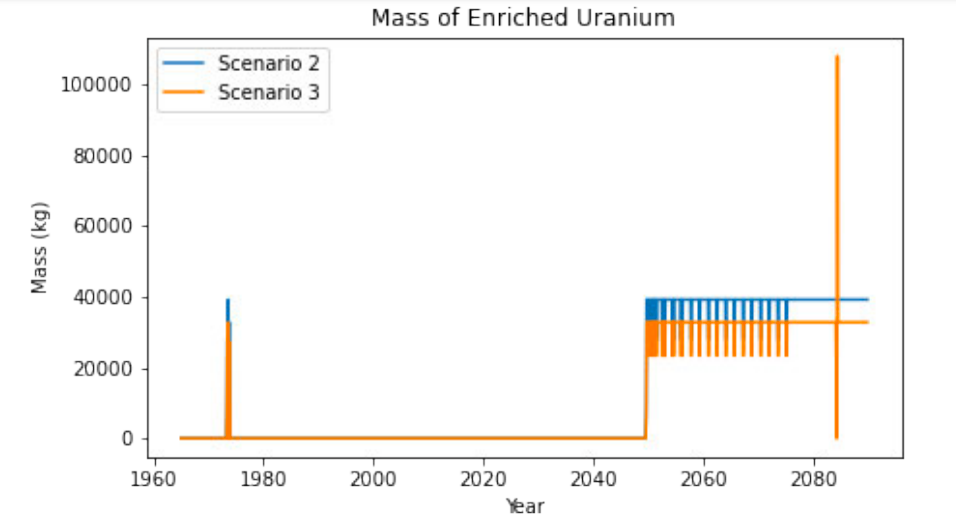
\includegraphics[height=2.7cm]{./images/mass.png}
                        \end{center}
                                \caption{Mass of Enriched Uranium.}
                        \label{fig:mass}
                \end{figure}
                \column[t]{5cm}
                \begin{figure}[htbp!]
                        \begin{center}
                                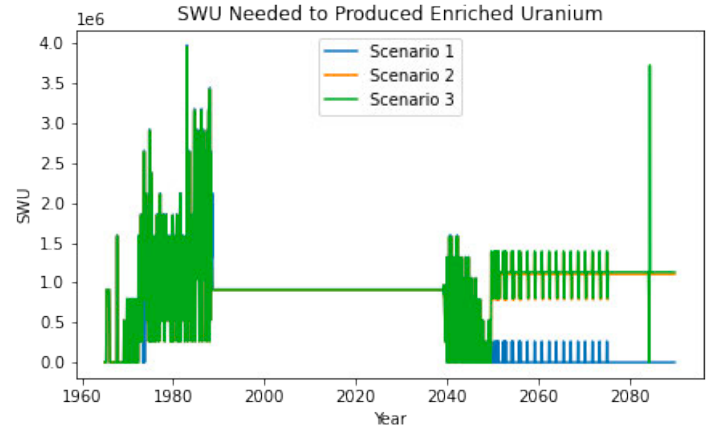
\includegraphics[height=3cm]{./images/swu.png}
                        \end{center}
                                \caption{Seperative Work Units needed for enrichment.}
                        \label{fig:swu}
                \end{figure}
              \end{columns}
\end{frame}


\begin{frame}
        \frametitle{Conclusions and Energy Use}
        % a comment
              \begin{columns}
                      \column[t]{5cm}
                        \begin{itemize}
                                \item Transition will require a mixture of HALEU production methods and deployments
                                \item Scenario 2 never reaches required power level
                                \item Scenario 3 requires more SWU than 2 due to higher enrichment
                        \end{itemize}
                      \column[t]{5cm}
              \begin{figure}[htbp!]
              \begin{center}
            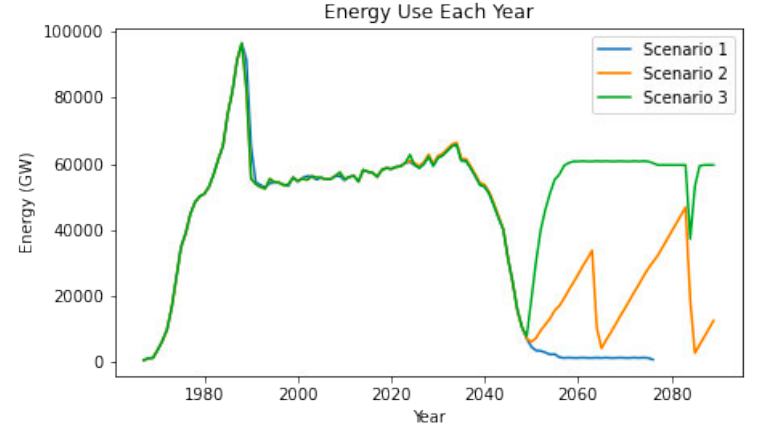
\includegraphics[height=3cm]{./images/e_use.png}
          \end{center}
                \caption{Energy use in each year. \cite{bachmann}}
          \label{fig:e_use}
        \end{figure}
              \end{columns}
\end{frame}
